\subsection{Explicación formal del problema}

\subsection{Explicación de la solución}

\subsection{Complejidad del algoritmo}

El análisis de complejidad es simple, es un algoritmo de Divide \& Conquer clásico, que divide siempre el trabajo en 2 y luego fusiona los resultados de los subproblemas en tiempo $O(n)$. Haciendo una analogía, por ejemplo, con el algoritmo de MergeSort, se puede predecir fácilmente que la complejidad será de $O(nlogn)$.

\subsubsection{Esbozo del algoritmo}

El algoritmo fue analizado en profundidad anteriormente. A grandes rasgos, puede describirse de la siguiente manera:
\begin{algorithm}
\begin{algorithmic}
\caption{Esbozo del algoritmo de KaioKen}
  \Procedure{generarpeleas}{int $n$, int $pactual$, int $inicio$}
  \If {$n = 1$}
    \State $matrizpeleas[pactual][inicio] \gets 1$
  \EndIf
  \If {$n = 2$}
    \State $matrizpeleas[pactual][inicio] \gets 1$
    \State $matrizpeleas[pactual][inicio + 1] \gets 2$
  \Else
    \For {$j \in [0,..., n)$}
      \If {$j < \frac{n}{2}$}
        \State $matrizpeleas[pactual][inicio + j] \gets 1$
      \Else 
        \State $matrizpeleas[pactual][inicio + j] \gets 2$
      \EndIf
    \EndFor
    \State $generarpeleas(\frac{n}{2}, pactual+1, inicio)$
    \State $generarpeleas(\frac{n+1}{2}, pactual+1, n/2 + inicio)$
  \EndIf
  \EndProcedure
\end{algorithmic}
\end{algorithm}

Como puede verse claramente, tenemos dos casos base que toman tiempo constante en ser resueltos.

Por otro lado, el tercer caso realiza un trabajo de costo lineal, escribiendo $n$ entradas de la matriz, y luego hace 2 llamadas recursivas, dividiendo el trabajo en 2 mitades iguales (en caso de que $n$ sea impar, la segunda mitad va a tener un elemento más).

\subsubsection{Análisis temporal}
Si quisieramos expresar la cantidad de operaciones que realiza el algoritmo para un input de tamaño $n$, podriamos escribirlo fácilmente de la siguiente manera:
\[T(1) = 1\]
\[T(2) = 2\]
\[T(n) = n + 2 T \left(\frac{n}{2}\right)\]

Ahora podemos usar el teorema maestro. El teorema maestro se referia a relaciones de recurrencia de la pinta:

\[T(n) = f(n) + a T\left(\frac{n}{b}\right)\]

Y afirmaba, entre otras cosas, que si $f(n) \in O(n^c log^k n)$ donde $c = log_b a$, entonces $T(n) \in \Theta(n^c log^{k+1} n)$. En este caso, se ve claramente que $f(n) = n \in O(n^1 log^0 n)$, y además $1 = log_2 2$, por lo que el teorema maestro se puede aplicar, y nos dice que

\[T(n) \in \Theta(n log n)\]

La complejidad de este algoritmo es siempre $\Theta(n logn)$, sin distinción entre casos, es decir, este algoritmo no tiene mejor o peor caso. La forma más clara de verlo es que el único input del problema es $n$, y no hay otro parámetro que pueda modificar su complejidad.

\subsection{Performance del algoritmo}

Como dijimos antes, la complejidad del algoritmo es siempre $\Theta(n logn)$, sin distinción entre casos, por lo que el análisis de performance es simple.

\begin{figure}[H]
 \centering
	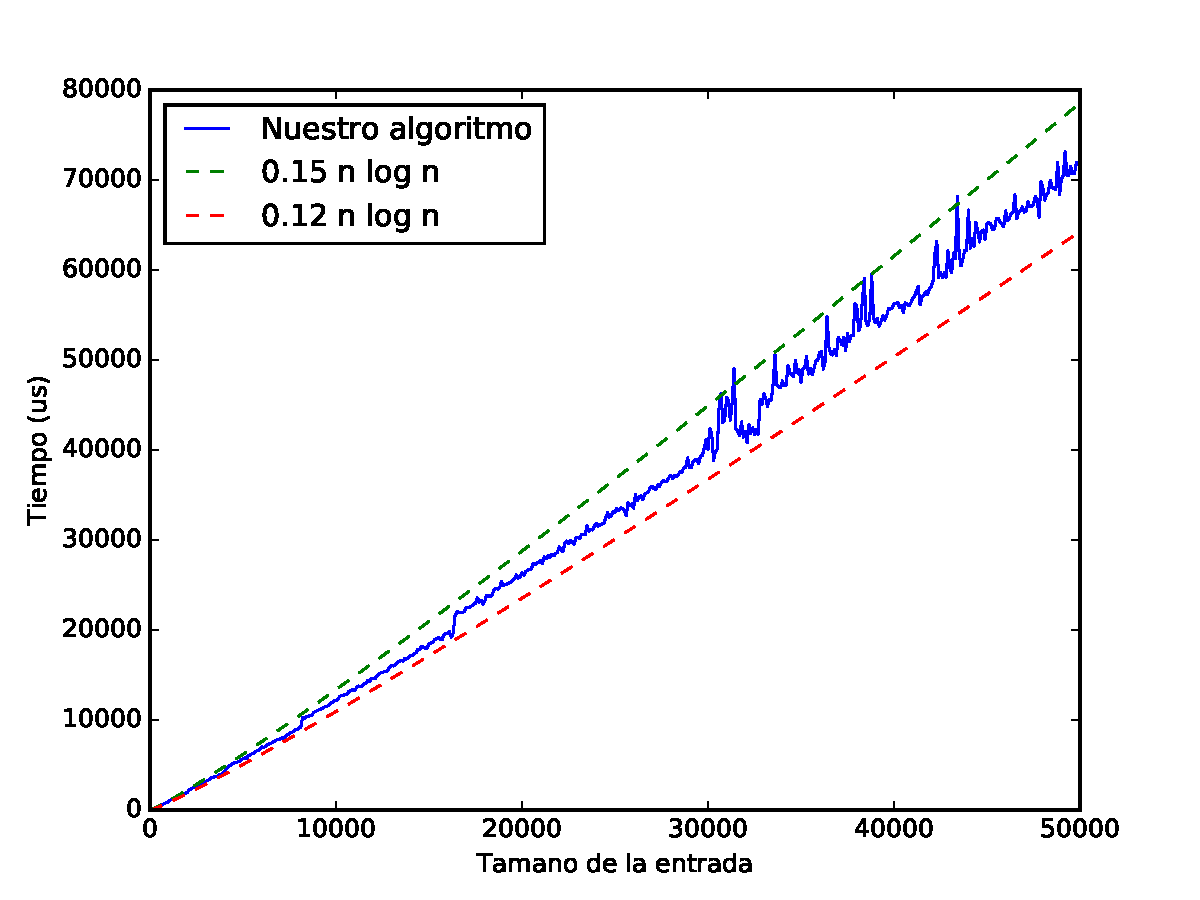
\includegraphics[width=0.7\textwidth]{img/tiempos/kaioken3.pdf}
	\caption{\footnotesize asdfg.}
	\label{fig:kaioken-tiempos3}
\end{figure}

\begin{figure}[H]
 \centering
	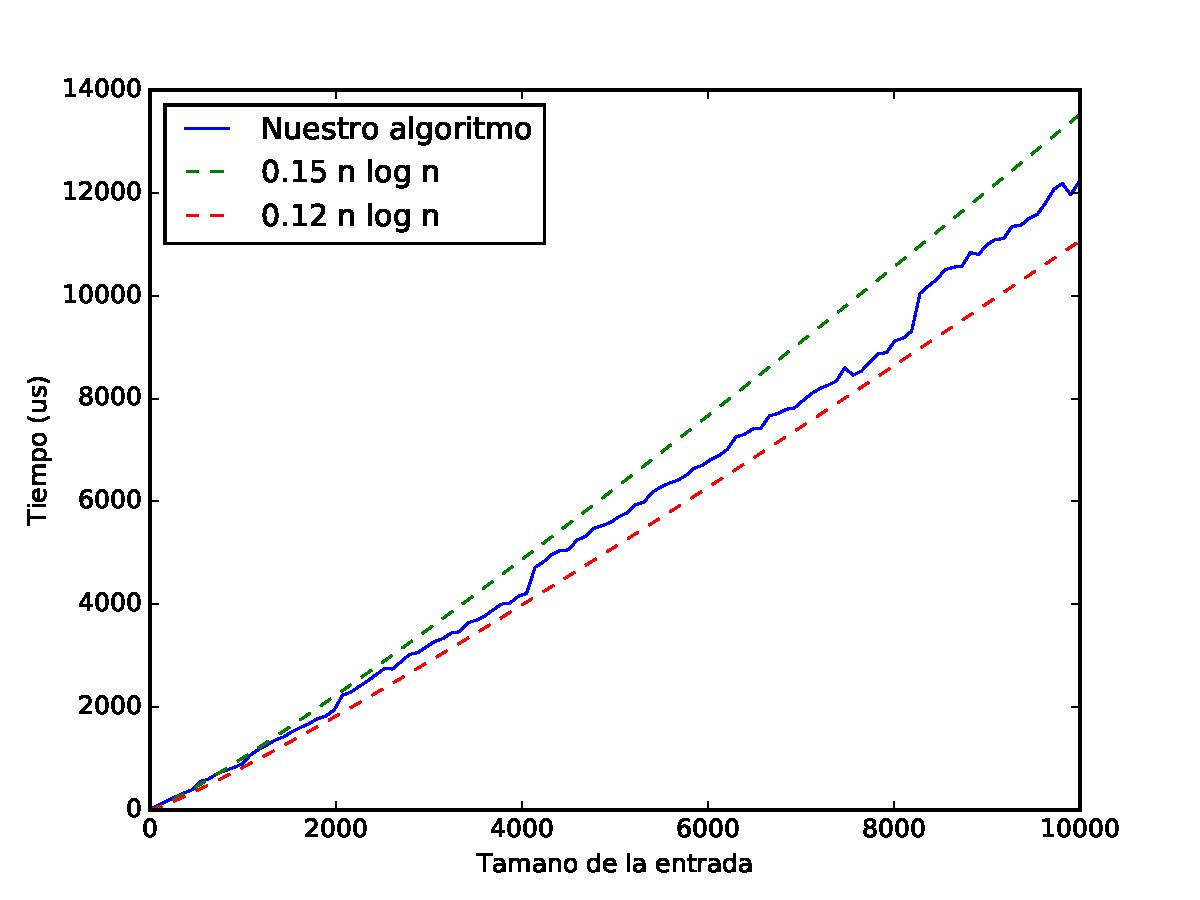
\includegraphics[width=0.7\textwidth]{img/tiempos/kaioken1.pdf}
	\caption{\footnotesize asdfg.}
	\label{fig:kaioken-tiempos1}
\end{figure}

\begin{figure}[H]
 \centering
	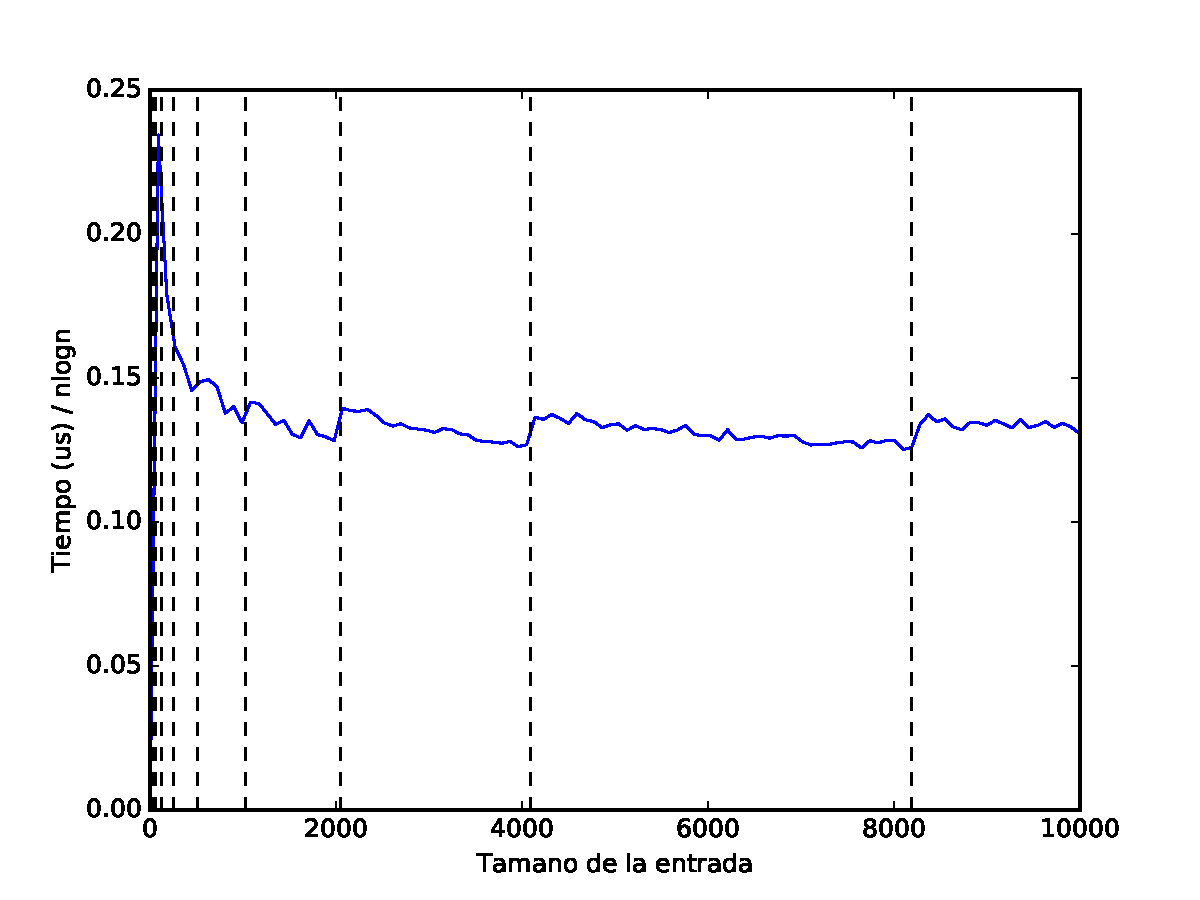
\includegraphics[width=0.7\textwidth]{img/tiempos/kaioken2.pdf}
	\caption{\footnotesize asdfg.}
	\label{fig:kaioken-tiempos2}
\end{figure}
